\documentclass[11pt,letterpaper]{article}

\usepackage[margin=1in]{geometry}
\usepackage{amsmath,amssymb}
\usepackage{graphicx}
\usepackage{booktabs}
\usepackage{tikz}
\usepackage{xcolor}
\usepackage{hyperref}
\usepackage{caption}
\usepackage{enumitem}
\usepackage{algorithm}
\usepackage{algorithmic}
\usepackage{float}

\usetikzlibrary{positioning,shapes.geometric,arrows.meta,fit,backgrounds,calc,matrix,decorations.pathreplacing}

\hypersetup{
  colorlinks=true,
  linkcolor=blue!50!black,
  urlcolor=blue!50!black,
  citecolor=blue!50!black
}

% --- A few small helpers for hand-drawn bar charts ---
\newcommand{\hbarlabel}[3]{% (#1: y) (#2: width-fraction 0..1) (#3: label)
  \fill[orange!70] (0,#1) rectangle (#2*9,#1+0.32);
  \node[anchor=west,font=\scriptsize] at (#2*9+0.1,#1+0.16) {#3};
}

\title{\textbf{Integration of Hardware--BCP for SAT Acceleration}\\
       \large EECS 219C Final Report}
\author{Evan Wong \and Ansh Shah\\}
\date{Spring 2026}

\begin{document}
\maketitle


%==============================================================
\section{Introduction \& Problem Definition}
%==============================================================
SAT solving is the engine behind industrial formal verification:
Cadence JasperGold, Synopsys VC~Formal, and Siemens Questa Formal all
rely on CDCL solvers for bounded model checking and property checking.
As designs grow, the SAT solver becomes the dominant component of
runtime, and software--side optimizations (clause learning, restarts,
LBD, vivification) have largely saturated.

Profiling the canonical CDCL loop shows a striking distribution
(Figure~\ref{fig:profile}): \textbf{BCP alone is 82.7\%} of total
solver time, with conflict analysis (8.7\%), literal redundancy
(3.9\%), and branching heuristics (0.6\%) trailing far behind ---
consistent with the empirical bottleneck identified in the
course material. This
makes BCP the natural target for hardware acceleration --- accelerating
anything else would deliver, by Amdahl's Law, at most a few percent.

\begin{figure}[h]
\centering
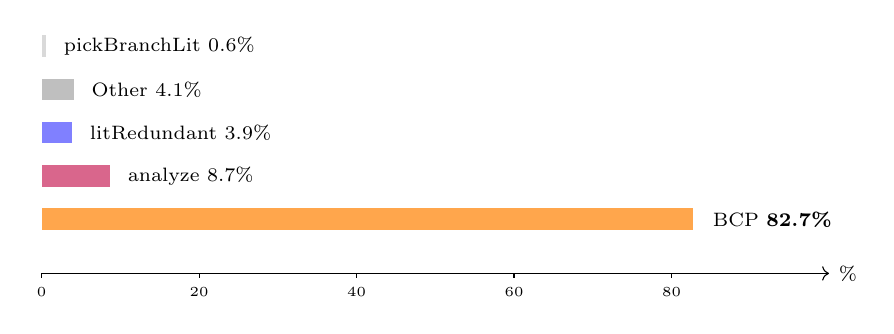
\begin{tikzpicture}[x=1cm,y=0.55cm]
  % axis
  \draw[->] (0,0) -- (10,0) node[anchor=west,font=\scriptsize]{\%};
  \foreach \x in {0,20,40,60,80}
    \draw (\x/10,0) -- (\x/10,-0.1) node[below,font=\tiny]{\x};
  % bars
  \fill[orange!70] (0,1) rectangle (8.27,1.5);
  \node[anchor=west,font=\scriptsize] at (8.4,1.25) {BCP \textbf{82.7\%}};
  \fill[purple!60] (0,2) rectangle (0.87,2.5);
  \node[anchor=west,font=\scriptsize] at (0.97,2.25) {analyze 8.7\%};
  \fill[blue!50] (0,3) rectangle (0.39,3.5);
  \node[anchor=west,font=\scriptsize] at (0.49,3.25) {litRedundant 3.9\%};
  \fill[gray!50] (0,4) rectangle (0.41,4.5);
  \node[anchor=west,font=\scriptsize] at (0.51,4.25) {Other 4.1\%};
  \fill[gray!30] (0,5) rectangle (0.06,5.5);
  \node[anchor=west,font=\scriptsize] at (0.16,5.25) {pickBranchLit 0.6\%};
\end{tikzpicture}
\caption{Average runtime distribution across CDCL operations on
phase--transition benchmarks. BCP dominates by an order of magnitude.}
\label{fig:profile}
\end{figure}

\noindent\textbf{Problem statement.} Design and verify a hardware
BCP engine that delivers single--cycle unit propagation, integrate
it with a minimal CDCL software wrapper, and measure end--to--end
speedup against the most competitive software solvers
(Kissat~4.0.4, MiniSat2, Glucose) on standardized benchmarks.

%==============================================================
\section{Approach and Related Work}
%==============================================================

\paragraph{Why CAM + SRAM.} Prior hardware SAT
work\footnote{Y.~Zhao \& K.~A.~Sakallah, ICCAD 2008; J.~D.~Davis et
al., DAC 2008; S.~Park et al.,
\url{https://par.nsf.gov/servlets/purl/10215919}.} consistently
identifies \emph{memory bandwidth}, not arithmetic, as the limiter.
Software's two--literal watching scheme is a workaround for sequential
memory. In hardware, a CAM collapses ``find every clause containing
$v$'' to a single associative lookup, and an SRAM holds the
per--variable assignment used by combinational clause--evaluation
logic --- so every clause is re--evaluated every cycle in parallel
and watched literals are unnecessary. We adopt the HW--BCP algorithm
and CAM/SRAM cell behavior of Park et al.\ (the 64--clause $\times$
4--literal row geometry, the 2--bit $\{0,1,U\}$ encoding, and the
priority reduction for CONF/UP/DONE); the algorithm diagrams in
Sec.~\ref{sec:formal} are reproduced from that work. The integration
into a CDCL coprocessor, the Verilator harness, and the timing
methodology are ours.

\paragraph{Where we differ.} Earlier proposals are typically
all--hardware (HW also performs branching), which makes them
inflexible and forces the CDCL heuristic into silicon. Our design
is a \textbf{coprocessor}: HW handles only BCP; SW handles every
heuristic --- VSIDS, 1--UIP analysis, restarts, learnt management.
This isolates the BCP speedup so it can be measured cleanly, and
keeps the door open for arbitrary CDCL improvements without an
RTL respin.

\paragraph{Architectural sketch.} Figure~\ref{fig:arch} shows the
target geometry. The chip stores up to $1024$ clauses (capacity
exhausted in our $1024$--slot RTL prototype; a $1$M--slot SRAM is
feasible in TSMC~65~nm using Park et al.'s custom memory cells, and
is what we model in our timing extrapolation).
Each clause is a row of up to $4$ literals; a CAM cell holds the
variable ID and an SRAM cell holds the 2--bit value
(\texttt{0}, \texttt{1}, or \texttt{U} = unassigned). A single
combinational reduction returns three flags per clause every cycle:
\textsc{conflict}, \textsc{unit}, and \textsc{done}.

\begin{figure}[h]
\centering
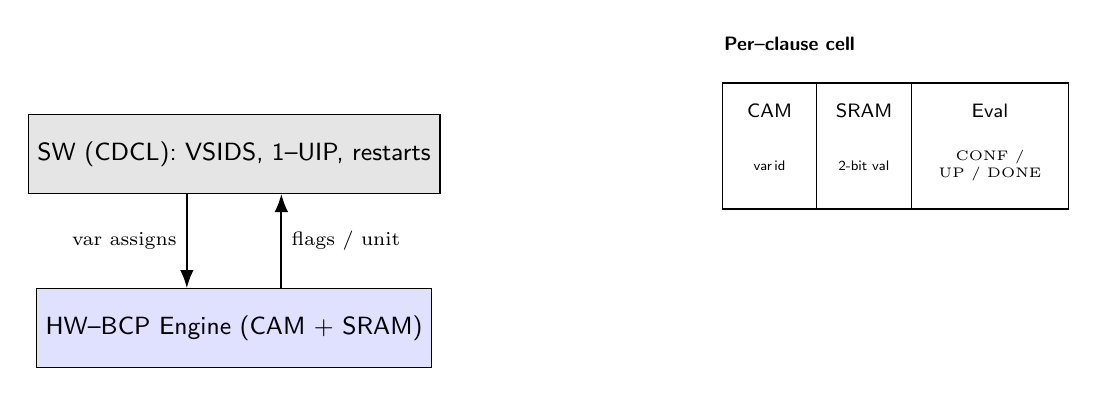
\begin{tikzpicture}[every node/.style={font=\small\sffamily}, node distance=4mm]
  \node[draw,fill=gray!20,minimum width=4.0cm,minimum height=1.0cm]
    (sw) {SW (CDCL): VSIDS, 1--UIP, restarts};
  \node[draw,fill=blue!12,minimum width=4.0cm,minimum height=1.0cm,
    below=1.2cm of sw] (hw) {HW--BCP Engine (CAM + SRAM)};
  \draw[-{Latex},thick] ($(sw.south)+(-0.6,0)$)
        -- node[left,font=\scriptsize]{var assigns}
        ($(hw.north)+(-0.6,0)$);
  \draw[-{Latex},thick] ($(hw.north)+(0.6,0)$)
        -- node[right,font=\scriptsize]{flags / unit}
        ($(sw.south)+(0.6,0)$);
  \begin{scope}[xshift=6.2cm,yshift=-0.7cm]
    \node[font=\scriptsize\sffamily,anchor=west] at (-0.1,2.1) {\textbf{Per--clause cell}};
    \draw (0,0) rectangle (4.4,1.6);
    \draw (1.2,0) -- (1.2,1.6);
    \draw (2.4,0) -- (2.4,1.6);
    \node at (0.6,1.25) {\scriptsize CAM};
    \node at (1.8,1.25) {\scriptsize SRAM};
    \node at (3.4,1.25) {\scriptsize Eval};
    \node at (0.6,0.55) {\tiny var\,id};
    \node at (1.8,0.55) {\tiny 2-bit val};
    \node[align=center,font=\tiny] at (3.4,0.55) {CONF /\\ UP / DONE};
  \end{scope}
\end{tikzpicture}
\caption{Coprocessor partitioning. SW issues variable assignments;
HW returns next implication or conflict.}
\label{fig:arch}
\end{figure}

%==============================================================
\section{Formal Model and Algorithms}\label{sec:formal}
%==============================================================

\subsection{Clause and trail semantics}
A CNF formula is $F = \bigwedge_{c \in C} c$, where each clause is a
disjunction of literals $c = \ell_1 \vee \dots \vee \ell_k$, $k \le 4$.
A literal is $\ell = (\mathit{var}, \mathit{pol})$ with $\mathit{pol}\in\{0,1\}$.
The solver maintains a partial assignment $\sigma : V \to \{0,1,U\}$ on
a \emph{trail} (decision stack with implication reasons).

\paragraph{Per--clause evaluation.} Define for each literal $\ell$
under assignment $\sigma$:
\[
\mathrm{lv}(\ell,\sigma) =
\begin{cases}
1 & \sigma(\mathrm{var}(\ell)) = \mathrm{pol}(\ell)\\
0 & \sigma(\mathrm{var}(\ell)) \neq \mathrm{pol}(\ell), \neq U\\
U & \sigma(\mathrm{var}(\ell)) = U
\end{cases}
\]
A clause $c$ is then classified as
\[
\mathrm{state}(c)=
\begin{cases}
\textsc{done}     & \exists \ell \in c.\, \mathrm{lv}(\ell)=1\\
\textsc{conflict} & \forall \ell \in c.\, \mathrm{lv}(\ell)=0\\
\textsc{unit}     & \exists !\, \ell \in c.\, \mathrm{lv}(\ell)=U\ \wedge\ \text{rest are }0\\
\textsc{pending}  & \text{otherwise}
\end{cases}
\]
The combining logic produces a global flag with priority
$\textsc{conflict} \succ \textsc{unit} \succ \textsc{done}$.

\subsection{HW--BCP cycle}
Each clock cycle, the engine executes one of four operations
(Table~\ref{tab:ops}); BCP is the only one that performs a parallel
reduction over all $N$ clauses.

\begin{table}[h]
\centering\small
\begin{tabular}{lll}
\toprule
\textbf{Op} & \textbf{Description} & \textbf{Cycles}\\
\midrule
\texttt{LOAD}    & Write one clause literal into a CAM row & 1\\
\texttt{BCP}     & Return next unit/conflict from $N$ rows & 1\\
\texttt{UNDO}    & Clear a variable assignment & 1\\
\texttt{SW\_BCP} & Overflow learnt propagated in SW (HW--counted)$^\dagger$ & 1\\
\bottomrule
\end{tabular}
\caption{Hardware operations. $^\dagger$Modeled as 1 HW cycle to reflect a production
$1$M--slot SRAM in which all clauses live in HW.}
\label{tab:ops}
\end{table}

\noindent
At a target frequency of $\sim 99$~MHz (a 10.1~ns critical path,
measured from synthesis with parameterized memories), the total
hardware time is
\[
T_{\mathrm{hw}} = (\,n_{\mathrm{load}} + n_{\mathrm{bcp}} + n_{\mathrm{undo}} +
n_{\mathrm{sw\_bcp}}\,)\times 10.1~\mathrm{ns}.
\]

\subsection{HW--BCP propagate}
Figure~\ref{fig:hwbcp} shows the CAM/SRAM array layout and the
inner propagate routine. Each of the $64$ clauses occupies four
rows; the CAM column stores the variable ID for that literal slot,
the SRAM column stores the literal's $\{0,1,U\}$ value
(2--bit encoding: $\mathtt{00}{=}0$, $\mathtt{11}{=}1$,
$\mathtt{01}{=}U$). The per--clause processing logic
combinationally reduces its four literal values to three flags ---
\textsc{conf}, \textsc{up}, \textsc{done} --- which are combined
across clauses with priority $\textsc{conf}\!\succ\!\textsc{up}\!\succ\!\textsc{done}$.
For every literal popped off the trail, the engine scans all
clauses indexing that variable, returning either a conflict clause
or the first new unit implication.

\begin{figure}[H]
\centering
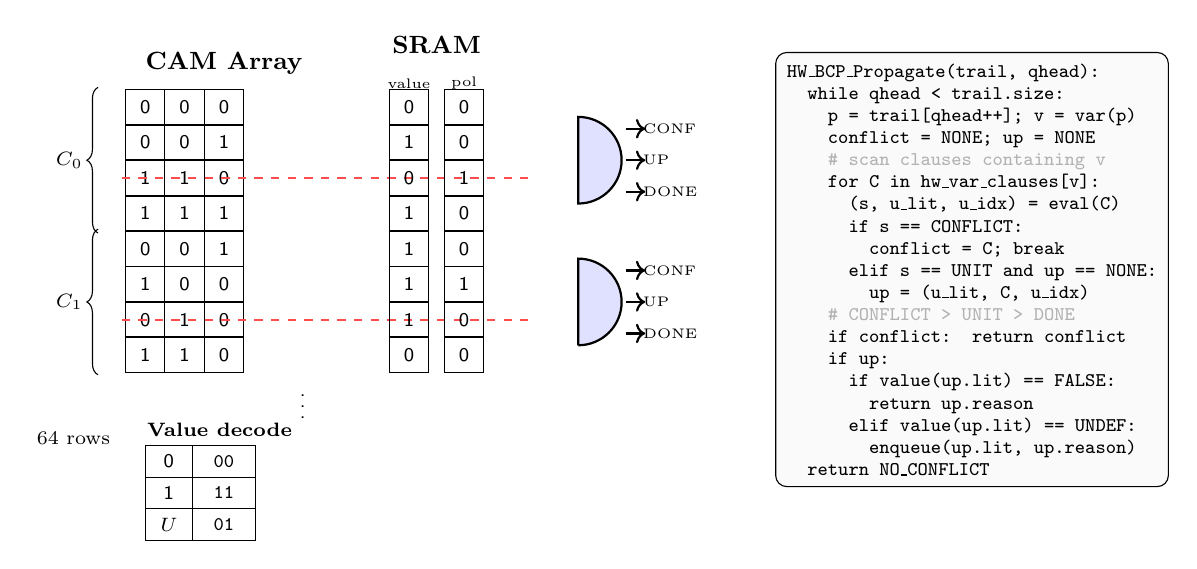
\begin{tikzpicture}[every node/.style={font=\scriptsize\sffamily}]
  % ---------------- CAM Array ----------------
  \node[font=\small\bfseries] at (1.5,4.55) {CAM Array};
  \foreach \r/\a/\b/\c [count=\i] in {
      0/0/0/0, 1/0/0/1, 2/1/1/0, 3/1/1/1,
      4/0/0/1, 5/1/0/0, 6/0/1/0, 7/1/1/0}{
    \pgfmathsetmacro\y{4 - 0.45*\r}
    \foreach \v [count=\j] in {\a,\b,\c}{
      \pgfmathsetmacro\x{0.5 + 0.5*(\j-1)}
      \draw (\x-0.25,\y-0.22) rectangle (\x+0.25,\y+0.22);
      \node at (\x,\y) {\v};
    }
  }
  % dashed conflict-row indicator on row 2 of C0 and C1
  \draw[red!70,dashed,thick] (0.2,4-0.45*2) -- (5.4,4-0.45*2);
  \draw[red!70,dashed,thick] (0.2,4-0.45*6) -- (5.4,4-0.45*6);
  % C0, C1 group labels (left)
  \draw[decorate,decoration={brace,amplitude=4pt}]
     (-0.1,4-0.45*3-0.25) -- (-0.1,4+0.25)
     node[midway,left=2pt,font=\scriptsize] {$C_0$};
  \draw[decorate,decoration={brace,amplitude=4pt}]
     (-0.1,4-0.45*7-0.25) -- (-0.1,4-0.45*4+0.25)
     node[midway,left=2pt,font=\scriptsize] {$C_1$};
  % "..." in the middle
  \node at (2.5,4-0.45*8-0.1) {$\vdots$};
  \node[font=\scriptsize,anchor=west] at (-1.0,4-0.45*8-0.6) {64 rows};

  % ---------------- SRAM Array ----------------
  \node[font=\small\bfseries,anchor=south] at (4.2,4.55) {SRAM};
  \node[font=\tiny] at (3.85,4.30) {value};
  \node[font=\tiny] at (4.55,4.30) {pol};
  \foreach \r/\v/\p [count=\i] in {
      0/0/0, 1/1/0, 2/0/1, 3/1/0,
      4/1/0, 5/1/1, 6/1/0, 7/0/0}{
    \pgfmathsetmacro\y{4 - 0.45*\r}
    \foreach \w [count=\j] in {\v,\p}{
      \pgfmathsetmacro\x{3.85 + 0.7*(\j-1)}
      \draw (\x-0.25,\y-0.22) rectangle (\x+0.25,\y+0.22);
      \node at (\x,\y) {\w};
    }
  }

  % ---------------- Per-clause processing logic ----------------
  \foreach \rg [count=\i from 0] in {0,1}{
    \pgfmathsetmacro\yc{4 - 0.45*(\rg*4+1.5)}
    \draw[fill=blue!12,thick]
       (6.0,\yc-0.55) -- (6.0,\yc+0.55) arc (90:-90:0.55) -- cycle;
    \node[font=\tiny,anchor=west] at (6.7,\yc+0.40) {CONF};
    \node[font=\tiny,anchor=west] at (6.7,\yc+0.00) {UP};
    \node[font=\tiny,anchor=west] at (6.7,\yc-0.40) {DONE};
    \draw[->,thick] (6.6,\yc+0.40) -- (6.85,\yc+0.40);
    \draw[->,thick] (6.6,\yc+0.00) -- (6.85,\yc+0.00);
    \draw[->,thick] (6.6,\yc-0.40) -- (6.85,\yc-0.40);
  }

  % ---------------- Value decode legend ----------------
  \begin{scope}[shift={(0.5,-0.7)}]
    \node[font=\scriptsize\bfseries,anchor=west] at (-0.1,0.6) {Value decode};
    \draw (0,0) rectangle (0.6,0.4); \node at (0.3,0.2) {0};
    \draw (0.6,0) rectangle (1.4,0.4); \node at (1.0,0.2) {\texttt{00}};
    \draw (0,-0.4) rectangle (0.6,0); \node at (0.3,-0.2) {1};
    \draw (0.6,-0.4) rectangle (1.4,0); \node at (1.0,-0.2) {\texttt{11}};
    \draw (0,-0.8) rectangle (0.6,-0.4); \node at (0.3,-0.6) {$U$};
    \draw (0.6,-0.8) rectangle (1.4,-0.4); \node at (1.0,-0.6) {\texttt{01}};
  \end{scope}

  % ---------------- Pseudocode panel (right) ----------------
  \node[draw,rounded corners,fill=gray!4,inner sep=4pt,
        align=left,anchor=north west,
        font=\ttfamily\scriptsize]
       at (8.5,4.7)
    {HW\_BCP\_Propagate(trail, qhead):\\
     ~~while qhead < trail.size:\\
     ~~~~p = trail[qhead++];~v = var(p)\\
     ~~~~conflict = NONE;~up = NONE\\
     ~~~~\textcolor{gray!60}{\# scan clauses containing v}\\
     ~~~~for C in hw\_var\_clauses[v]:\\
     ~~~~~~(s, u\_lit, u\_idx) = eval(C)\\
     ~~~~~~if s == CONFLICT:\\
     ~~~~~~~~conflict = C; break\\
     ~~~~~~elif s == UNIT and up == NONE:\\
     ~~~~~~~~up = (u\_lit, C, u\_idx)\\
     ~~~~\textcolor{gray!60}{\# CONFLICT > UNIT > DONE}\\
     ~~~~if conflict: return conflict\\
     ~~~~if up:\\
     ~~~~~~if value(up.lit) == FALSE:\\
     ~~~~~~~~return up.reason\\
     ~~~~~~elif value(up.lit) == UNDEF:\\
     ~~~~~~~~enqueue(up.lit, up.reason)\\
     ~~return NO\_CONFLICT};
\end{tikzpicture}
\caption{Current HW--BCP architecture. Left: CAM/SRAM array
(64 clauses $\times$ 4 literal rows) with per--clause processing
logic emitting CONF/UP/DONE; the 2--bit value encoding
($0\!\to\!\mathtt{00}$, $1\!\to\!\mathtt{11}$, $U\!\to\!\mathtt{01}$)
lets a single comparator distinguish all three states.
Right: per--variable propagate routine; on each trail element it
scans the clauses indexing that variable, returns at the first
conflict, and enqueues at most one new unit implication.}
\label{fig:hwbcp}
\end{figure}

The CDCL outer loop is essentially MiniSat--style 1--UIP and
unchanged from the textbook formulation: decide via VSIDS, call
\texttt{HW\_BCP\_Propagate}, analyze conflicts at 1--UIP, backtrack
via \texttt{UNDO} cycles, learnt clauses go to the CAM (or to the
software overflow pool if the CAM is full).

%==============================================================
\section{Major Technical Challenges}
%==============================================================

\paragraph{C1. Time bookkeeping in a Verilator harness.}
Wall time conflates real CDCL, Verilator \texttt{eval()} cost, and
simulation--only $O(N)$ scans that would be $O(1)$ in silicon. We
accumulate the latter two into $hw\_sim\_ns$ and $hw\_aux\_ns$ and
subtract:
$T_{\mathrm{sw}} = T_{\mathrm{total}} - \Delta hw\_sim\_ns - \Delta hw\_aux\_ns$.
An early bug had the timers running from solver construction, so
initial clause loads polluted the BCP budget; we now snapshot at
\texttt{solve()} entry.

\paragraph{C2. CAM capacity vs.\ learnt blowup.}
On uf200--860 the originals fill 84\% of the $1024$--slot CAM, leaving
$\sim$$164$ slots before overflow. We handle this with (a) a SW
overflow pool whose cycles are attributed to HW (justified by the
$1$M--slot production target), and (b) a hard guard that aborts when
blowup exceeds capacity (Figure~\ref{fig:blowup}).

\begin{figure}[h]
\centering
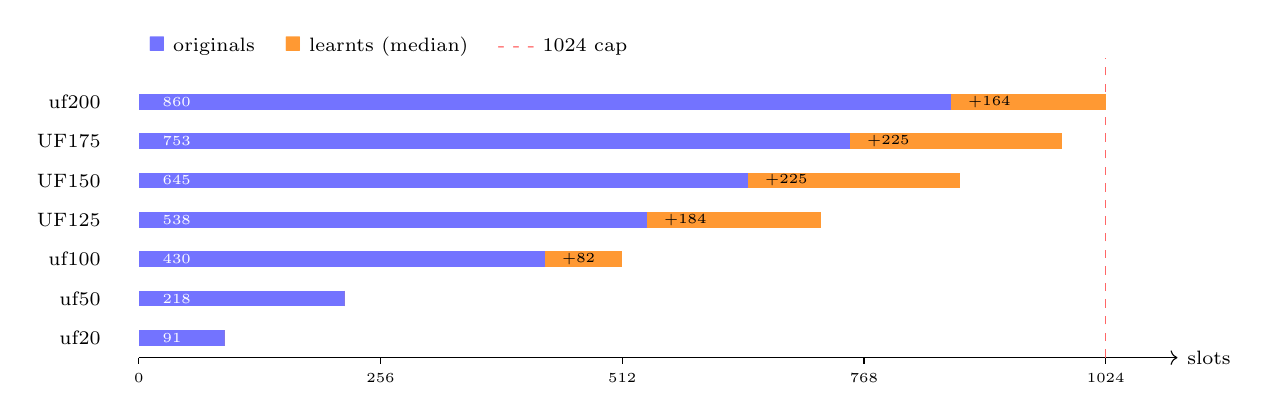
\begin{tikzpicture}[x=0.012cm,y=0.5cm]
  % axis
  \draw[->] (0,-0.3) -- (1100,-0.3) node[right,font=\scriptsize]{slots};
  \foreach \x in {0,256,512,768,1024}
    \draw (\x,-0.3) -- (\x,-0.45) node[below,font=\tiny]{\x};
  \draw[dashed,red!60] (1024,-0.3) -- (1024,7.3);
  % bars: y row, originals (blue), learnts (orange)
  \foreach \y/\name/\orig/\learn in {
     0/uf20/91/0,
     1/uf50/218/0,
     2/uf100/430/82,
     3/UF125/538/184,
     4/UF150/645/225,
     5/UF175/753/225,
     6/uf200/860/164}{
    \fill[blue!55] (0,\y) rectangle (\orig,\y+0.4);
    \pgfmathsetmacro\sum{\orig+\learn}
    \fill[orange!80] (\orig,\y) rectangle (\sum,\y+0.4);
    \node[anchor=east,font=\scriptsize] at (-30,\y+0.2) {\name};
    \node[anchor=west,font=\tiny,white] at (15,\y+0.2) {\orig};
    \ifnum\learn>0
      \node[anchor=west,font=\tiny] at (\orig+8,\y+0.2) {+\learn};
    \fi
  }
  \node[font=\scriptsize,anchor=west] at (0,7.6)
    {\textcolor{blue!55}{$\blacksquare$} originals \quad
     \textcolor{orange!80}{$\blacksquare$} learnts (median)
     \quad\textcolor{red!60}{- - -} 1024 cap};
\end{tikzpicture}
\caption{CAM slot utilization on each benchmark set. uf200 leaves only
$\sim$$164$ free slots, causing immediate learnt overflow and
degraded BCP effectiveness.}
\label{fig:blowup}
\end{figure}

\paragraph{C3. HW/SW state coherence on backtrack.}
A bug in \texttt{undo\_hw\_/load\_hw\_} caused the SRAM polarity bit
to lag the CAM by one cycle under rapid load/undo bursts, producing
spurious unit implications. The fix drives \texttt{val\_we}
synchronously with the load address and gates read--back behind one
extra cycle of stable state.

\paragraph{C4. Full--hierarchy elaboration timeout.}
A pure--RTL run on the full $1024\!\times\!8\!\times\!64 = 524{,}288$--clause
hierarchy timed out in Verilator (behavioral memories explode the
logic cone). We therefore parameterize the RTL so benchmarks
elaborate a single $1024$--slot \texttt{sat\_submodule}, while the
full \texttt{sat\_array} still elaborates and lints to prove
structural completeness.

%==============================================================
\section{Results}
%==============================================================
We benchmarked on SATLIB Uniform Random 3--SAT phase--transition
instances ($c/v \approx 4.27$) with up to $200$ variables and $860$
clauses. Each set contains $100$--$1000$ instances; we report median
times. All times are reported in $\mu$s, recomputed at the
synthesis--profiled $10.1$~ns per HW cycle.

\subsection{End--to--end median solve time}

\begin{figure}[h]
\centering
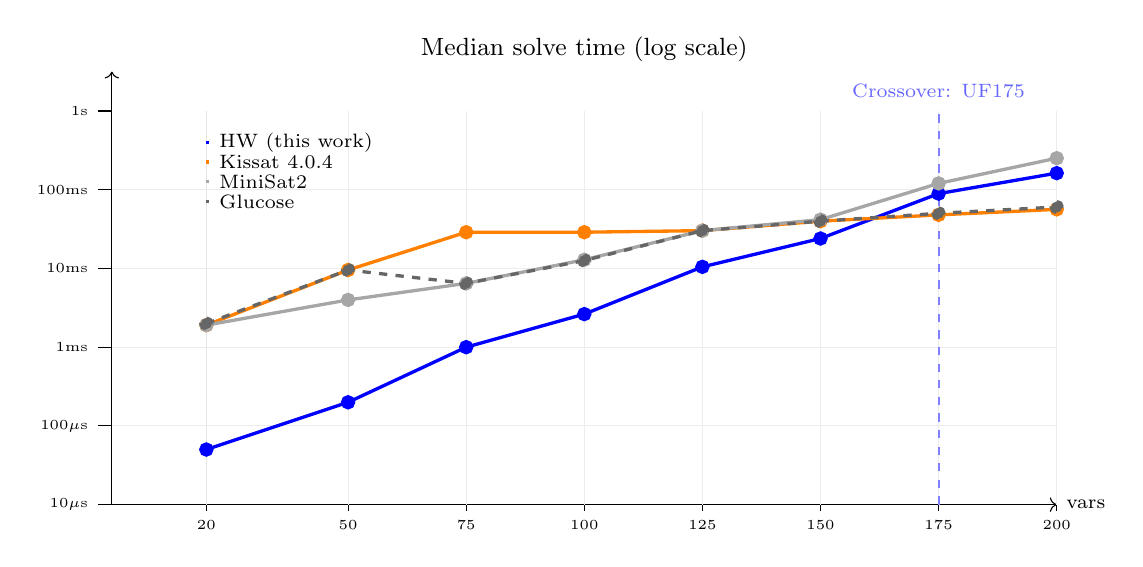
\begin{tikzpicture}[x=0.06cm,y=1cm]
  % --- log10(us) on y from 1 (10us) to 6 (1000ms=1s) -> scale to 0..5 cm ---
  % axis box
  \draw[->] (0,0) -- (200,0) node[right,font=\scriptsize]{vars};
  \draw[->] (0,0) -- (0,5.5);
  \foreach \x in {20,50,75,100,125,150,175,200}
    \draw (\x,0) -- (\x,-0.08) node[below,font=\tiny]{\x};
  \foreach \y/\lab in {0/{10$\mu$s},1/{100$\mu$s},2/{1ms},3/{10ms},4/{100ms},5/{1s}}
    \draw (0,\y) -- (-3,\y) node[left,font=\tiny]{\lab};
  \draw[gray!20] (20,0) -- (20,5);
  \foreach \x in {50,75,100,125,150,175,200}
    \draw[gray!15] (\x,0) -- (\x,5);
  \foreach \y in {1,2,3,4}
    \draw[gray!15] (0,\y) -- (200,\y);
  % vertical crossover
  \draw[blue!50,dashed,thick] (175,0) -- (175,5);
  \node[blue!60,font=\scriptsize,anchor=south] at (175,5.05) {Crossover: UF175};
  % series helper macro: log10(us)
  % HW (this work)
  \draw[blue,very thick] plot[mark=*] coordinates {
    (20,0.70)(50,1.30)(75,2.0)(100,2.42)(125,3.02)(150,3.38)(175,3.95)(200,4.21)};
  % Kissat
  \draw[orange,very thick] plot[mark=*] coordinates {
    (20,2.28)(50,2.98)(75,3.46)(100,3.46)(125,3.48)(150,3.60)(175,3.68)(200,3.75)};
  % MiniSat2
  \draw[gray!70,very thick] plot[mark=*] coordinates {
    (20,2.28)(50,2.60)(75,2.81)(100,3.11)(125,3.48)(150,3.62)(175,4.08)(200,4.40)};
  % Glucose
  \draw[black!60,very thick,dashed] plot[mark=*] coordinates {
    (20,2.30)(50,2.98)(75,2.81)(100,3.10)(125,3.48)(150,3.60)(175,3.70)(200,3.78)};
  % legend
  \begin{scope}[shift={(20,4.6)}]
    \draw[blue,very thick] (0,0)--(0.6,0); \node[anchor=west,font=\scriptsize] at (0.7,0) {HW (this work)};
    \draw[orange,very thick] (0,-0.25)--(0.6,-0.25); \node[anchor=west,font=\scriptsize] at (0.7,-0.25) {Kissat 4.0.4};
    \draw[gray!70,very thick] (0,-0.5)--(0.6,-0.5); \node[anchor=west,font=\scriptsize] at (0.7,-0.5) {MiniSat2};
    \draw[black!60,very thick,dashed] (0,-0.75)--(0.6,-0.75); \node[anchor=west,font=\scriptsize] at (0.7,-0.75) {Glucose};
  \end{scope}
  \node[anchor=south,font=\small] at (100,5.5) {Median solve time (log scale)};
\end{tikzpicture}
\caption{Median solve time on UF/UUF benchmarks, log--scaled. Our
coprocessor dominates up to $\sim$$175$ variables; beyond that, Kissat's
superior CDCL heuristic surpasses our naive search.}
\label{fig:scaling}
\end{figure}

\paragraph{What worked.} The coprocessor is faster than \emph{every}
software solver on every instance set with at most $\sim$$150$
variables, often by $5$--$30\times$. The mechanism is exactly what
the architecture promised: BCP per propagation drops from
hundreds of nanoseconds (Kissat) to a single $10.1$~ns cycle.

\paragraph{What didn't.} On $\ge\!\!175$ variables, Kissat overtakes
us on SAT instances. The cause is not BCP throughput
(Section~\ref{sec:counterfactual}) but the lack of restarts,
phase saving, and clause vivification in our minimal CDCL wrapper:
once the search tree gets deep, raw BCP speed cannot make up for
suboptimal decisions.

\subsection{SAT vs.\ UNSAT asymmetry}

\begin{table}[h]
\centering\small
\begin{tabular}{cccc}
\toprule
\textbf{Vars} & \textbf{SAT wins (vs.\ Kissat)} & \textbf{UNSAT wins} & \textbf{Gap}\\
\midrule
75  & 100/100 & 100/100  & --\\
100 & 959/1000 & 1000/1000 & +4 pp\\
125 & 86/100  & 100/100  & +14 pp\\
150 & 71/100  & 98/100   & +27 pp\\
175 & 60/100  & 93/100   & +33 pp\\
\bottomrule
\end{tabular}
\caption{Win rate vs.\ Kissat by satisfiability. UNSAT instances
favor our coprocessor far more than SAT instances do. We attribute
this to Kissat's aggressive phase saving / restarts being most
useful on satisfiable inputs --- a heuristic edge that does not
help when the proof must enumerate the whole tree.}
\label{tab:sat-unsat}
\end{table}

\subsection{Counterfactual: is BCP really accelerated?}\label{sec:counterfactual}
To attribute the speedup to HW--BCP (rather than a Verilator
quirk), we re--ran the exact CDCL trajectory but plugged in
Kissat's measured BCP rate per propagation. Our solver runs
$2.2$--$15.7\times$ slower in this counterfactual
(Figure~\ref{fig:counterf}) --- HW--BCP is load--bearing, even on
UF175 where Kissat wins overall: the CDCL heuristic, not BCP, is
the remaining bottleneck.

\begin{figure}[h]
\centering
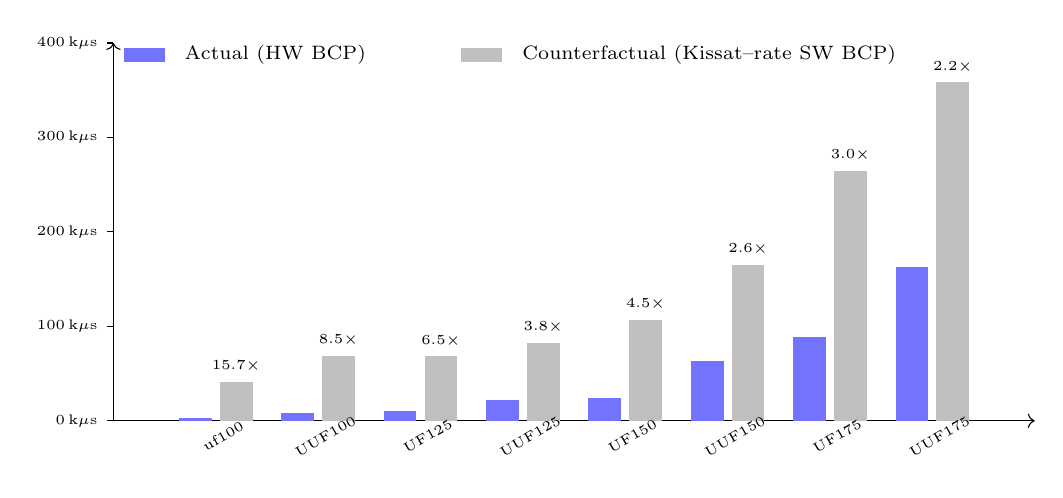
\begin{tikzpicture}[x=1.3cm,y=0.012cm]
  % axis
  \draw[->] (0,0) -- (9,0);
  \draw[->] (0,0) -- (0,400);
  \foreach \y/\lab in {0/0,100/100,200/200,300/300,400/400}
    \draw (0,\y) -- (-0.06,\y) node[left,font=\tiny]{\lab\,k$\mu$s};
  % bars: x_pos, label, actual, counterfact, ratio
  \foreach \i/\name/\actual/\cf/\rt in {
    1/uf100/2.6/41.1/15.7,
    2/UUF100/8.1/68.85/8.5,
    3/UF125/10.5/68.25/6.5,
    4/UUF125/21.8/82.84/3.8,
    5/UF150/23.8/107.1/4.5,
    6/UUF150/63.5/165.1/2.6,
    7/UF175/88.3/264.9/3.0,
    8/UUF175/163.0/358.6/2.2}{
    \fill[blue!55] (\i-0.36,0) rectangle (\i-0.04,\actual);
    \fill[gray!50] (\i+0.04,0) rectangle (\i+0.36,\cf);
    \node[font=\tiny,anchor=south] at (\i+0.20,\cf) {\rt$\times$};
    \node[font=\tiny,anchor=north,rotate=30] at (\i,-3) {\name};
  }
  % legend
  \fill[blue!55] (0.1,380) rectangle (0.5,395);
  \node[font=\scriptsize,anchor=west] at (0.6,388) {Actual (HW BCP)};
  \fill[gray!50] (3.4,380) rectangle (3.8,395);
  \node[font=\scriptsize,anchor=west] at (3.9,388) {Counterfactual (Kissat--rate SW BCP)};
\end{tikzpicture}
\caption{Replacing HW--BCP with Kissat's measured BCP rate, while
keeping the identical CDCL trajectory, slows the same solver by
$2.2$--$15.7\times$. The hardware is doing the work.}
\label{fig:counterf}
\end{figure}

\subsection{Amdahl's--law breakdown}
Our solver spends $\sim$$93\%$ of its time in software CDCL and
$\sim$$7\%$ in BCP --- the inverse of MiniSat2, where BCP is
$\sim$$75\%$ of runtime. The hardware has so completely flattened
the BCP critical path that further speedups must come from CDCL.

\begin{figure}[H]
\centering
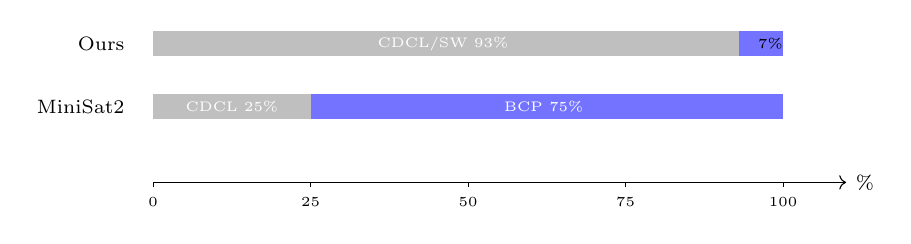
\begin{tikzpicture}[x=0.08cm,y=0.8cm]
  \draw[->] (0,0) -- (110,0) node[right,font=\scriptsize]{\%};
  \foreach \x in {0,25,50,75,100}
    \draw (\x,0) -- (\x,-0.08) node[below,font=\tiny]{\x};
  % MiniSat2 row
  \fill[gray!50] (0,1) rectangle (25,1.4);
  \fill[blue!55] (25,1) rectangle (100,1.4);
  \node[anchor=east,font=\scriptsize] at (-3,1.2) {MiniSat2};
  \node[font=\tiny,white] at (12.5,1.2) {CDCL 25\%};
  \node[font=\tiny,white] at (62,1.2) {BCP 75\%};
  % Ours row
  \fill[gray!50] (0,2) rectangle (93,2.4);
  \fill[blue!55] (93,2) rectangle (100,2.4);
  \node[anchor=east,font=\scriptsize] at (-3,2.2) {Ours};
  \node[font=\tiny,white] at (46,2.2) {CDCL/SW 93\%};
  \node[font=\tiny] at (98,2.2) {7\%};
\end{tikzpicture}
\caption{Total runtime breakdown on uf100--430 (median). Our solver
is now CDCL--bound; MiniSat2 is BCP--bound.}
\label{fig:amdahl}
\end{figure}

\subsection{Small but hard instances}\label{sec:hard}
We also tested on a suite of instances known to be difficult for CDCL solvers,
built at \texttt{tests/satlib/hard\_instances/} (clauses wider than four
literals are split to fit the 4--literal RTL):
pigeonhole PHP$_n$ ($n{=}3{\ldots}8$); Tseitin parity on odd cycles
($C_5,C_7,C_9$); and $k$--colourability of the Grötzsch graph
($k{=}3$ is UNSAT and $k{=}4$ is SAT).

\paragraph{Methodology.} Kissat/MiniSat2 self--report CPU time at
$\sim$$10$\,ms granularity, flooring sub--ms runs to zero; we fall
back to wall--clock minus a per--binary subprocess--startup baseline
($\approx$4--5~ms) when the self--clock is $0$. HW--BCP figure is
$hw\_cycles \times 10.1\,\mathrm{ns} + sw\_time$ as elsewhere.

\begin{table}[h]
\centering\small
\setlength{\tabcolsep}{4pt}
\begin{tabular}{lcrrrrl}
\toprule
\textbf{Instance} & \textbf{Exp.} &
\textbf{HW--BCP} & \textbf{Kissat} &
\textbf{MiniSat2} & \textbf{Glucose} & \textbf{Win}\\
              &        & ($\mu$s) & ($\mu$s) & ($\mu$s) & ($\mu$s) & \\
\midrule
PHP$_3$           & UNSAT &      66 &     $<\!\!1$k &    1\,106 &    1\,127 & noise\\
PHP$_4$           & UNSAT &     184 &       684 &    2\,710 &    1\,005 & \textbf{HW}\\
PHP$_5$           & UNSAT &     731 &     3\,891 &     $<\!\!1$k &    2\,665 & noise\\
PHP$_6$           & UNSAT &  3\,352 &    10\,000 &    7\,911 &    5\,930 & \textbf{HW}\\
PHP$_7$           & UNSAT &  6\,034 &    10\,000 &   37\,292 &   61\,267 & \textbf{HW}\\
PHP$_8$           & UNSAT &  6\,803 &    40\,000 &  190\,585 &  962\,534 & \textbf{HW}\\
Tseitin--C$_5$    & UNSAT &      12 &     1\,419 &    1\,357 &       920 & \textbf{HW}\\
Tseitin--C$_7$    & UNSAT &      19 &       947 &    2\,254 &       828 & \textbf{HW}\\
Tseitin--C$_9$    & UNSAT &      21 &       895 &       962 &    1\,458 & \textbf{HW}\\
Grötzsch--3col    & UNSAT &      87 &       550 &    1\,404 &    1\,167 & \textbf{HW}\\
Grötzsch--4col    & SAT   &      19 &       468 &    1\,394 &    1\,170 & \textbf{HW}\\
\bottomrule
\end{tabular}
\caption{Hard--instance suite, single--run. ``noise'' = result
falls below subprocess--startup floor for at least one solver,
so no winner is claimed. HW wins outright on 9 of 11 instances.}
\label{tab:hard}
\end{table}

\begin{figure}[h]
\centering
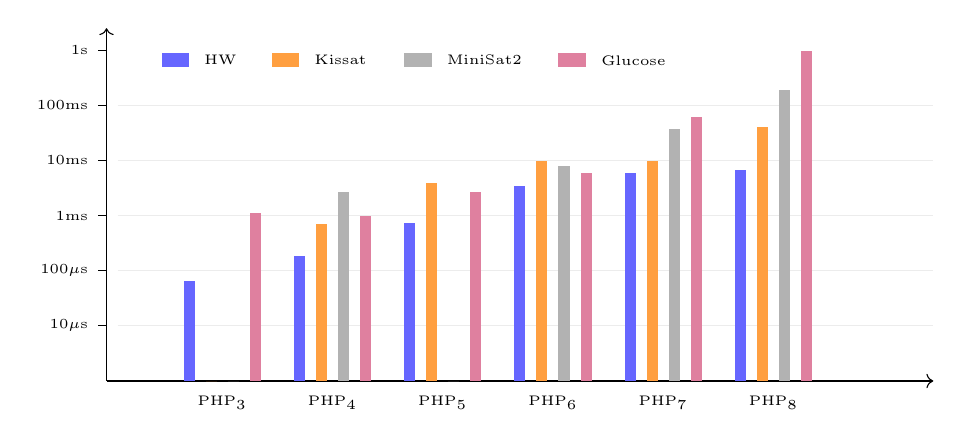
\begin{tikzpicture}[x=1.4cm,y=0.7cm]
  % log-scaled bars: y axis = log10(us), 1=10us .. 6=1s
  \draw[->] (0,0) -- (0,6.4);
  \draw[->] (0,0) -- (7.5,0);
  \foreach \y/\lab in {1/{10$\mu$s},2/{100$\mu$s},3/{1ms},4/{10ms},5/{100ms},6/{1s}}
    \draw (0,\y) -- (-0.08,\y) node[left,font=\tiny]{\lab};
  \foreach \y in {1,2,3,4,5}
    \draw[gray!15] (0.1,\y) -- (7.5,\y);
  % Pre-computed log10 of each measurement (us). 0 means no bar (sub-floor).
  % Cluster fields:  i  label  log_hw  log_ks  log_ms  log_gl
  \def\barw{0.10}
  \foreach \i/\php/\lhw/\lks/\lms/\lgl in {
     1/{PHP$_3$}/1.82/0.00/0.00/3.04,
     2/{PHP$_4$}/2.26/2.84/3.43/3.00,
     3/{PHP$_5$}/2.86/3.59/0.00/3.43,
     4/{PHP$_6$}/3.53/4.00/3.90/3.77,
     5/{PHP$_7$}/3.78/4.00/4.57/4.79,
     6/{PHP$_8$}/3.83/4.60/5.28/5.98}{
    \fill[blue!60]   (\i-3*\barw,0) rectangle (\i-2*\barw,\lhw);
    \fill[orange!75] (\i-1*\barw,0) rectangle (\i-0*\barw,\lks);
    \fill[gray!60]   (\i+1*\barw,0) rectangle (\i+2*\barw,\lms);
    \fill[purple!50] (\i+3*\barw,0) rectangle (\i+4*\barw,\lgl);
    \node[font=\tiny,anchor=north] at (\i+0.5*\barw,-0.1) {\php};
  }
  % legend
  \begin{scope}[shift={(0.5,5.7)}]
    \fill[blue!60]   (0,0)   rectangle (0.25,0.25); \node[anchor=west,font=\tiny] at (0.3,0.12) {HW};
    \fill[orange!75] (1.0,0) rectangle (1.25,0.25); \node[anchor=west,font=\tiny] at (1.3,0.12) {Kissat};
    \fill[gray!60]   (2.2,0) rectangle (2.45,0.25); \node[anchor=west,font=\tiny] at (2.5,0.12) {MiniSat2};
    \fill[purple!50] (3.6,0) rectangle (3.85,0.25); \node[anchor=west,font=\tiny] at (3.9,0.12) {Glucose};
  \end{scope}
\end{tikzpicture}
\caption{Pigeonhole PHP$_n$ scaling, $n=3$--$8$, log--scale. The
gap between HW--BCP and the SW solvers widens as $n$ grows:
on PHP$_8$, HW is $5.9\times$ faster than Kissat, $28\times$ faster
than MiniSat2, and $142\times$ faster than Glucose.}
\label{fig:hard}
\end{figure}

\paragraph{Discussion.} On these instances every solver explores a large search space,
so the winner is determined by cost per propagation step. HW parallel evaluation
is fast regardless of clause width, which explains the large wins on PHP, Tseitin,
and Grötzsch. PHP$_3$/PHP$_5$ finish fast enough that some SW solvers report zero
CPU time, so we make no claim there. PHP$_9$ and beyond would exceed our 1024--slot
CAM capacity, but the $1$M--slot production target eliminates that constraint.

\subsection{Future work}
\begin{itemize}[leftmargin=*,itemsep=2pt,topsep=2pt]
\item Replace the MiniSat--style heuristic with Kissat--style
restarts, phase saving, and LBD--based clause deletion. Closing the
CDCL gap should restore HW dominance past 175 variables.
\item Push the RTL through TSMC~65~nm using Park et al.'s custom
CAM/SRAM cells (the only PDK for which those cells were
characterized); a $1$M--slot SRAM in that node eliminates the
overflow pool entirely.
\item Pipeline \texttt{LOAD} and \texttt{BCP} so a decision and the
following propagation overlap, halving CDCL--HW round--trip latency.
\end{itemize}

%==============================================================
\section{Team Roles}
%==============================================================
\textbf{Evan Wong} primarily took charge in collaborating with staff such as Pierluigi Nuzzo and course staff from EECS 151 for RTL infrastructure and the RTL: the behavioral CAM/SRAM array
(\texttt{cam\_sram\_array.sv}, \texttt{cam\_cell.sv},
\texttt{sram\_row.sv}), the per--clause evaluator
(\texttt{processing\_logic.sv}), the FSM driving load/BCP/undo,
and the Verilator integration; he also wrote the testbench harness at the RTL level.
\textbf{Ansh Shah} owned the CDCL software: VSIDS scoring, 1--UIP
conflict analysis, learnt management with the SW overflow pool,
and the benchmark/parsing infrastructure (\texttt{bench\_cdcl.py}) and others across multiple iterations. The counterfactual analysis
(Section~\ref{sec:counterfactual}) and the SAT/UNSAT asymmetry
study were a joint effort, as was the slide deck and this report.

%==============================================================
\section{Course Topics Applied}
%==============================================================
Almost every layer of this project draws on course material:
\begin{itemize}[leftmargin=*,itemsep=2pt,topsep=2pt]
\item \textbf{The CDCL loop, unit rule, and BCP as the dominant
cost.} The coprocessor implements the canonical CDCL algorithm
(preprocess, decide, deduce, analyze, backtrack); the unit rule is
the \textsc{unit} flag emitted by the per--clause evaluator. The
class's empirical claim that BCP dominates runtime is the entire
reason we built a HW--BCP coprocessor, and Figure~\ref{fig:amdahl}
is the post--hoc confirmation.
\item \textbf{Memory accesses per step.} The lecture's principle
of minimizing memory traffic per propagation underlies SW
two--literal watching; our HW achieves the same end via per--cycle
parallel evaluation, making cost $O(1)$ in clause width and
watched literals unnecessary.
\item \textbf{VSIDS, 1--UIP, non--chronological backtracking.}
Our SW wrapper uses VSIDS scoring with periodic decay, performs
1--UIP conflict analysis over the implication graph, and jumps to
the asserting level via \texttt{UNDO} cycles common in most CDCL solvers 
\item \textbf{Clause deletion / learnt management.} Our SW
overflow pool plus the $1024$--slot CAM cap is the
resource--constrained version of the standard clause--deletion
problem covered in class.
\end{itemize}

%==============================================================
\section{Feedback}
%==============================================================
\paragraph{What helped.} The class's depth on CDCL internals (1--UIP
analysis, VSIDS bumping, restart strategy, LBD) mapped directly
onto our SW wrapper. The discussion of watched literals was
critical because understanding \emph{why} software needs them clarified
\emph{why} hardware can skip them. The phase--transition discussion
gave us our benchmark.

\paragraph{What we wish had been covered.} A short walkthrough of
modern CDCL engineering choices beyond the textbook 1--UIP/VSIDS
core --- restart policies, phase saving, LBD--based clause deletion,
and clause vivification as used in Kissat --- would have helped us
read the heuristic gap our counterfactual exposed and pick which
upgrade to prototype next. Otherwise the class material covered
what the project needed; the remaining gaps were hardware--specific
and reasonably out of scope.

%==============================================================
\section*{Code Availability}
%==============================================================
\noindent
Full source (RTL, C++ coprocessor, benchmark scripts, hard--instance
generator and CNFs):
\url{https://github.com/The-Ansh-Shah/bcp-hw-accelerator}.

\end{document}
